%template1.tex
%The following LaTeX source file represents the simplest kind of slide presentation; no overlays, no included graphics. Substitute your favorite style for ``pascal''. To create the PDF file template1.pdf, (1) be sure to use the prosper class, then (2) execute the command latex template1.tex, and (3) the command dvipdf template1.dvi.

%%%%%%%%%%%%%%%%%%%%%%%%%%%%%%% template1.tex %%%%%%%%%%%%%%%%%%%%%%%%%%%%%%%%%%%
\documentclass[a4paper,blends,pdf,colorBG,slideColor]{prosper}
% definitions for slides for CSC544
% Lutz Hamel, (c) 2007

\hypersetup{pdfpagemode=FullScreen}

\usepackage{times}
\usepackage{latexsym}
\usepackage{alltt}
\usepackage{booktabs}
\usepackage{amsmath}
\usepackage{amsopn}
\usepackage{amsfonts}
\usepackage{amssymb}
%\usepackage[usenames]{color}

\def\sign{\qopname\relax{no}{sign}}
\def\argmax{\qopname\relax{no}{argmax}}
\def\argmin{\qopname\relax{no}{argmin}}

\newcommand{\grad}{\ensuremath{\nabla}} 
\newcommand{\loss}{\ensuremath{{\cal L}}}
\newcommand{\err}{\mbox{err}}
\newcommand{\mse}{\mbox{mse}}
\newcommand{\acc}{\mbox{acc}}
\newcommand{\Integer}{\ensuremath{\mathbb{N}}}
\newcommand{\size}[1]{{|{#1}|}}
\newcommand{\Rnspace}[1]{\ensuremath{\mathbb{R}^{#1}}}
\newcommand{\Real}{\ensuremath{\mathbb{R}}}
\newcommand{\mytt}[1]{{\small\tt{#1}}}
\newcommand{\textemph}[1]{{\em #1}}
\newcommand{\suchthat}{\mid}
\newcommand{\orbar}{\;|\;}
\newcommand{\bs}[1]{\begin{slide}{#1}\ptsize{8}}
\newcommand{\es}{\end{slide}}
\newcommand{\co}{\,\colon\;}
\newcommand{\pair}[2]{\ensuremath{( {#1}, {#2} )}}
\newcommand{\model}[1]{\hat{#1}}
\newcommand{\ul}[1]{{\bf\em #1}}
\newcommand{\ol}{\overline}
\newcommand{\definition}[1]{{\bf Definition: }{\em #1}}
\newcommand{\example}[1]{{\bf Example: }{#1}}
\newcommand{\abs}[1]{|{#1}|}
\newcommand{\mytab}{\makebox[.1in]{}}

\newcommand{\fdef}[1]{
\begin{center}
\fbox{
\begin{minipage}{3.5in}
{\bf Definition:}
{#1}
\end{minipage}
}
\end{center}
}

\newcommand{\fframe}[1]{
\begin{center}
\fbox{
\begin{minipage}{3.5in}
{#1}
\end{minipage}
}
\end{center}
}

\newcommand{\nframe}[1]{
\begin{center}
\begin{minipage}{3.5in}
{#1}
\end{minipage}
\end{center}
}

\newenvironment{Rcode}
	{
		\scriptsize
		\begin{quote}
		\begin{alltt}
	}
	{
		\end{alltt}
		\end{quote}
	}




\begin{document}

\bs{Decision Surfaces \& Functions}
For some decision surface $g(\ol{x})=\ol{w}\bullet\ol{x} = b$ in an $n$-dimensional dot product space $\Rnspace{n}$ we can always construct the decision function,
 \begin{equation*}
\model{f}(\ol{x}) = \left\{
\begin{array}{ll}
+1 & \mbox{if $g(\ol{x}) -b \ge 0$,}\\
-1 & \mbox{if $g(\ol{x})-b < 0$,}
\end{array}
\right.
\end{equation*}
for all $\ol{x}\in \Rnspace{n}$.
Or in more compact form,

\begin{equation*}
\label{eq:linear-decision-function}
\framebox{$\model{f}(\ol{x}) = \sign(\ol{w}\bullet\ol{x} - b),$}
\end{equation*}
with $\ol{w}, \ol{x}\in \Rnspace{n}$, $b \in \mathbb{R}$, and
 \begin{equation*}
\sign(k) = \left\{
\begin{array}{ll}
+1 & \mbox{if $k \ge 0$,}\\
-1 & \mbox{if $k < 0$,}
\end{array}
\right.
\end{equation*}
for all $k \in \Real$.

\es



\bs{A Simple Learning Algorithm}
Let's investigate a simple algorithm that actually computes a decision surface for our  training set 
\begin{equation*}
D = \{\pair{\ol{x}_1}{y_1},\pair{\ol{x}_2}{y_2},\ldots,\pair{\ol{x}_l}{y_l}\},
\end{equation*}
with $\ol{x}_i \in \Rnspace{2}$ and $y_i \in \{+1, -1\}$.
 Here we relax the restriction that the decision surface has to go through the origin but
 we still assume that $D$ is linearly separable.
\begin{center}
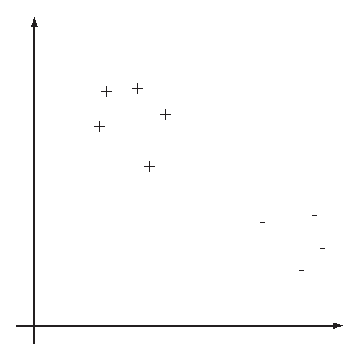
\includegraphics[height=45mm]{figures/simple-data.eps}
\end{center}
\es

\bs{A Simple Learning Algorithm}
{\bf Step 1.}

Compute the mean vectors,  $\ol{c}_+$ and $\ol{c}_-$, for each class, respectively:
\begin{eqnarray*}
\ol{c}_+ & = & \frac{1}{l_+}\sum_{(\ol{x}_i,+1)\in D} \ol{x}_i,\\
\ol{c}_- & = & \frac{1}{l_-}\sum_{(\ol{x}_i,-1)\in D} \ol{x}_i,
\end{eqnarray*}
where 
\begin{eqnarray*}
l_+ &=& \size{\{(\ol{x},y) \suchthat (\ol{x},y) \in D \text{ and } y = +1\}},\\
l_- &=& \size{\{(\ol{x},y) \suchthat (\ol{x},y) \in D \text{ and } y = -1\}}.
\end{eqnarray*}
\es



\bs{A Simple Learning Algorithm}

\begin{center}
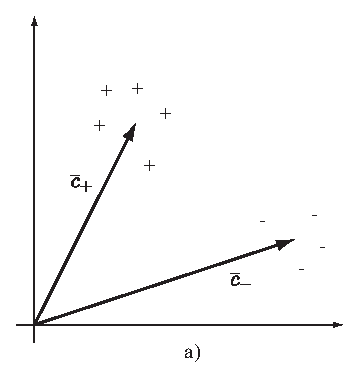
\includegraphics[height=60mm]{figures/simple-a.eps}
\end{center}
\es

\bs{A Simple Learning Algorithm}

{\bf Step 2.}

Next, we construct the vector $\ol{d}$ such that $\ol{c}_+ = \ol{c}_- + \ol{d}$ or,
\begin{equation*}
\ol{d} = \ol{c}_+ -\ol{c}_- .
\end{equation*}

\vspace{.2in}

\begin{center}
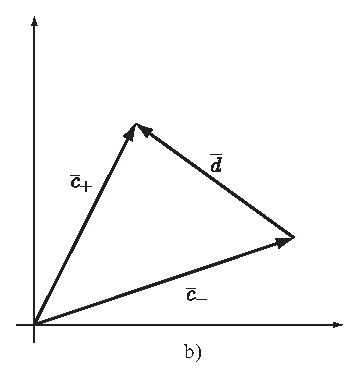
\includegraphics[height=45mm]{figures/simple-b.eps}
\end{center}
\es


\bs{A Simple Learning Algorithm}

{\bf Step 3.}

Compute the midpoint, $\ol{c}$, between the two means 
$\ol{c}_+$ and $\ol{c}_-$ such that
\[
\ol{c} = \frac{1}{2}(\ol{c}_+ + \ol{c}_-).
\]

\vspace{.2in}

\begin{center}
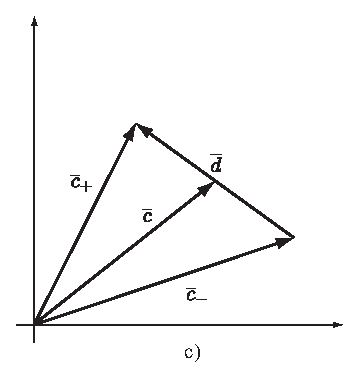
\includegraphics[height=45mm]{figures/simple-c.eps}
\end{center}
\es

\bs{A Simple Learning Algorithm}

{\bf Step 4.}

We translate the vector $\ol{d}$ so that it is rooted in the average object $\ol{c}$ and we construct
a line perpendicular to $\ol{d}$ through $\ol{c}$.
We can now interpret this line as a decision surface $\ol{w}\bullet\ol{x} = b$ with
with 
$\ol{w} = \ol{d}$ and
$b = \ol{d}\bullet\ol{c}$, graphically,

\vspace{.2in}
\begin{center}
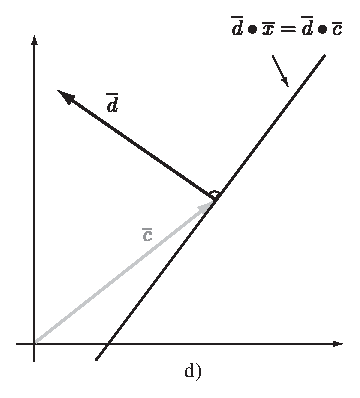
\includegraphics[height=45mm]{figures/simple-d.eps}
\end{center}
\es

\bs{A Simple Learning Algorithm}
Putting this all together.
\vspace{.2in}
\begin{center}
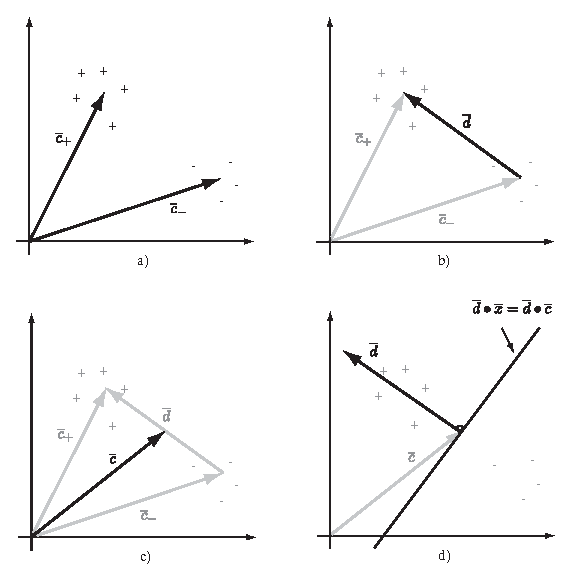
\includegraphics[height=60mm]{figures/fig04-03.eps}
\end{center}
\es

\bs{A Simple Learning Algorithm}

{\bf Step 5.}


Finally, given our decision surface above we obtain the model,
\begin{align*}
\model{f}(\ol{x}) &= \sign(\ol{d}\bullet\ol{x} - \ol{d}\bullet\ol{c})\\
	& = \sign\left ((\ol{x} - \ol{c})\bullet\ol{d}\right )\\
	& = \sign\left (\abs{\ol{x} - \ol{c}}\abs{\ol{d}}\cos \gamma\right ),
\end{align*}
for all $\ol{x} \in \Rnspace{2}$.
\es

\bs{A Simple Learning Algorithm}

We can illustrate this with a point $\ol{a}$,
\begin{equation*}
\model{f}(\ol{a}) = \sign\left (\abs{\ol{a} - \ol{c}}\abs{\ol{d}}\cos \gamma\right ),
\end{equation*}

\begin{minipage}{2in}
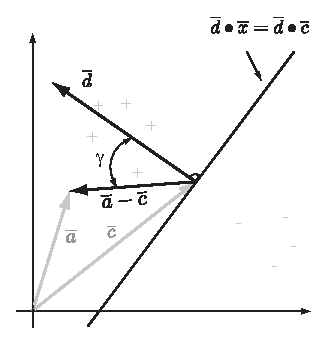
\includegraphics[height=50mm]{figures/fig04-04.eps}
\end{minipage}
\begin{minipage}{2in}
\begin{equation*}
\model{f}(\ol{a}) = \left\{
\begin{array}{ll}
+1 & \mbox{if $\gamma \le 90^\circ$}\\
-1 & \mbox{if $\gamma > 90^\circ$}
\end{array}
\right.
\end{equation*}
\end{minipage}

\es


\bs{A Simple Learning Algorithm}
We can derive an
algebraic form of our model from the definitions of $\ol{c}$ and $\ol{d}$,

\begin{align*}
\model{f}(\ol{x}) & = \sign \left ((\ol{x} - \ol{c})\bullet\ol{d}\right)\nonumber\\
	& = \sign \left ( \left [\ol{x} - \frac{1}{2}(\ol{c}_+ +\ol{c}_- ) \right ]\bullet(\ol{c}_+ - \ol{c}_-)\right).
\end{align*}
This shows that the model uses the class means in order to classify unknown points.
\es

\bs{A Simple Learning Algorithm}
{\bf Limitations.}

Outliers can distort the orientation of the decision surface which
leads to misclassification errors.  

\vspace{.2in}

\begin{center}
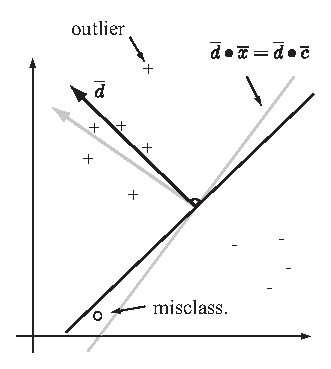
\includegraphics[height=50mm]{figures/fig04-05.eps}
\end{center}
\es

\end{document}
%%%%%%%%%%%%%%%%%%%%%%%%%%% end of template1.tex %%%%%%%%%%%%%%%%%%%%%%%%%%%%%%%%

